\section{669 --- Trim a Binary Search Tree}
Given a binary search tree and the lowest and highest boundaries as $L$ and $R$, trim the tree so that all its elements lies in $[L, R]$ ($R \geq L$). You might need to change the root of the tree, so the result should return the new root of the trimmed binary search tree.

\paragraph{Example 1:}

\begin{flushleft}


\textbf{Input}: $L = 1$, $R = 2$

\begin{figure}[H]
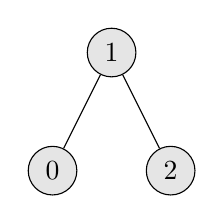
\begin{tikzpicture}
[every node/.style={draw, circle, fill=gray!20!, minimum size=5mm}]
\node{1}
child{node{0}}
child{node{2}};
\end{tikzpicture}
\end{figure}
 
\textbf{Output}: 

\begin{figure}[H]
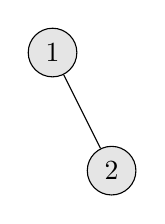
\begin{tikzpicture}
[every node/.style={draw, circle, fill=gray!20!, minimum size=5mm}]
\node{1}
child[missing]
child{node{2}};
\end{tikzpicture}
\end{figure}

\end{flushleft}

\paragraph{Example 2:}
\begin{flushleft}


\textbf{Input}:  $L = 1$,  $R = 3$
 
%    3
%   / \
%  0   4
%   \
%    2
%   /
%  1



\begin{figure}[H]
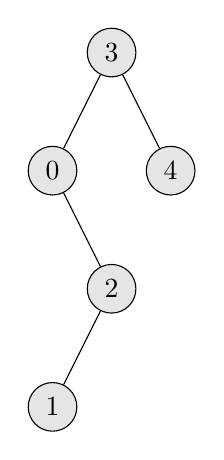
\begin{tikzpicture}
[every node/.style={draw, circle, fill=gray!20!, minimum size=5mm}]
\node{3}
child{node{0} child[missing] child{node{2} child{node{1}} child[missing] } }
child{node{4}};
\end{tikzpicture}
\end{figure}

\textbf{Output}:

\begin{figure}[H]
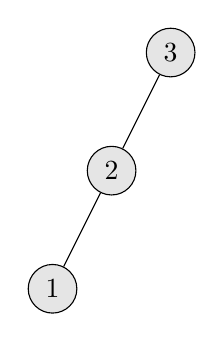
\begin{tikzpicture}
[every node/.style={draw, circle, fill=gray!20!, minimum size=5mm}]
\node{3}
child{node{2} child{node{1}} child[missing]}
child[missing];
\end{tikzpicture}
\end{figure} 
\end{flushleft}

\subsection{Recursion}
Since the given binary tree is a binary search tree, we know that 

\begin{itemize}
\item If root node's value $x$ is less than $L$, we will trim the right child tree.
\item If root node's value $x$ is larger than $R$, we will trim the left child tree.
\item If root node's value $x$ is in the range $[L, R]$, trim the left child tree for range $[L, x]$ and trim the right child tree for range $[x, R]$. The returned nodes will be the root's new left and right child.
\end{itemize}